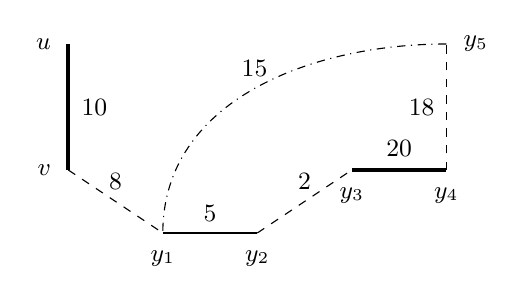
\begin{tikzpicture}[scale=.8]
\small

\coordinate (u) at (0, 1);
\coordinate (v) at (0, -1);
\coordinate (y1) at (1.5, -2);
\coordinate (y2) at (3, -2);
\coordinate (y3) at (4.5, -1);
\coordinate (y4) at (6, -1);
\coordinate (y5) at (6, 1);

\filledvertex{u}
\filledvertex{v}
\draw (u) node [left = 3pt] {$u$};
\draw (v) node [left = 3pt] {$v$};

\foreach \i in {1,...,4} {
    \filledvertex{y\i}
    \draw (y\i) node [below = 3pt] {$y_\i$};
}
\filledvertex{y5}
\draw (y5) node [right = 3pt] {$y_5$};

\draw[-, line width=.5mm] (u) -- node [right=1pt] {10} (v);
\draw[-, line width=.5mm] (y3) -- node [above=1pt] {20} (y4);
\draw[dashed] (v) -- node [above=1pt] {8} (y1);
\draw[-] (y1) -- node [above=1pt] {5} (y2);
\draw[dashed] (y2) -- node [above=1pt] {2} (y3);
\draw[dashed] (y4) -- node [left=1pt] {18} (y5);
\draw (y5) edge[dash dot,out=180, in=90] node[above=1pt] {15} (y1);

\end{tikzpicture}
